\documentclass[12pt]{article}
\usepackage{xeCJK}
\usepackage{fontspec}
\usepackage{amsmath}
\usepackage{graphicx}
\usepackage{geometry}
\usepackage{siunitx}
\usepackage{float}
\usepackage{fancyhdr}
\usepackage{circuitikz}
\setCJKmainfont{Songti SC}
\geometry{a4paper, margin=1in, top=1in}
\setlength{\parindent}{12pt}
% 页眉页脚设置
\pagestyle{fancy}
\fancyhf{}
\setlength{\headheight}{10pt}
%\fancyhead[L]{\raisebox{-0.5\height}{\includegraphics[width=0.15\textwidth]{pku_logo.png}}}
\fancyhead[R]{\small 普通物理实验报告}
\fancyhead[C]{\small 实验名称：分光计的调节和掠入射法测量折射率}
\fancyfoot[C]{\thepage}
\renewcommand{\headrulewidth}{0.4pt}

\title{\Large\textbf{分光计实验报告}}
\author{普通物理实验\\
        [REDACTED]\\
         \\
        姓名：\underline{\hspace{1cm}[REDACTED]\hspace{1cm}} \\
        学号：\underline{\hspace{0.5cm}[REDACTED]\hspace{0.5cm}} \\
        序号：\underline{\hspace{1.3cm}[REDACTED]\hspace{1.3cm}}}
\date{\today}

\begin{document}

\maketitle

%\section{实验目的}
%在此处填写实验目的...

%\section{实验器材}
%\begin{itemize}
%    \item 器材1
%    \item 器材2
%    \item 器材3
%\end{itemize}

%\section{实验原理}
%在此处说明实验原理...

%\section{实验步骤}
%\begin{enumerate}
%    \item 第一步...
%    \item 第二步...
%    \item 第三步...
%\end{enumerate}

\section{实验数据与分析}
\subsection{三棱镜顶角$A$的测量}
\begin{table}[H]
    \centering
    \begin{tabular}{cccccc}
        序号 & $\theta_1'$     & $\theta_1''$     & $\theta_2'$      & $\theta_2''$     & A                   \\ \hline
        1  & $40^{\circ}19'$ & $220^{\circ}19'$ & $160^{\circ}20'$ & $340^{\circ}18'$ & $60^{\circ}00'$     \\
        2  & $19^{\circ}24'$ & $199^{\circ}25'$ & $139^{\circ}25'$ & $319^{\circ}24'$ & $60^{\circ}00'$     \\
        3  & $42^{\circ}40'$ & $222^{\circ}39'$ & $162^{\circ}40'$ & $342^{\circ}38'$ & $60^{\circ}00'30''$
        \end{tabular}
    \caption{三棱镜顶角A测量数据}
\end{table}

\quad 根据实验数据，三棱镜顶角$A$的测量结果和A类不确定度如下：\\
\begin{align*}
    \overline{A} &= \frac{60^{\circ}00' + 60^{\circ}00' + 60^{\circ}00'30''}{3} = 60^{\circ}00'10'' \\
    u_A &= \sqrt{\frac{\sum_{i=1}^3(A_i-\overline{A})^2}{n(n-1)}} = 10'' \\
\end{align*}
\quad B类不确定度分析：
认为误差均匀分布，B类不确定度为仪器允许差的$1/\sqrt{3}$,即
\begin{equation*}
    u_{B1} = \frac{e}{\sqrt{3}} = \frac{1'}{\sqrt{3}}=35'' \\
\end{equation*}
\quad 合成不确定度：
\begin{equation*}
    u_c = \sqrt{u_A^2 + u_{B1}^2} \approx 36''
\end{equation*}
\quad 最终测量结果：
\begin{equation}
    A = 60^{\circ}00'10'' \pm 00^{\circ}00'36'' \\
\end{equation}    
\subsection{掠入射法测量三棱镜折射率}
\vspace{0.2cm}
\quad 采用钠灯作为光源，测量三棱镜对钠黄光$\lambda = 589.3\,nm$的折射率。实验数据如下：\\
\begin{table}[H]
    \centering
    \begin{tabular}{cccccc}
        序号 & $\theta_3'$     & $\theta_3''$     & $\theta_4'$      & $\theta_4''$     & A                   \\ \hline
        1  & $6^{\circ}24'$ & $186^{\circ}24'$ & $47^{\circ}48'$ & $227^{\circ}48'$ & $41^{\circ}24'$     \\
        2  & $358^{\circ}22'$($-360^{\circ}$) & $178^{\circ}21'$ & $39^{\circ}48'$ & $219^{\circ}47'$ & $41^{\circ}26'$     \\
        3  & $356^{\circ}9'$($-360^{\circ}$) & $176^{\circ}7'$ & $37^{\circ}34'$ & $217^{\circ}32'$ & $41^{\circ}25'$
        \end{tabular}
    \caption{极限角$\phi$测量数据}

\end{table}

\begin{figure}[H]
    \centering
    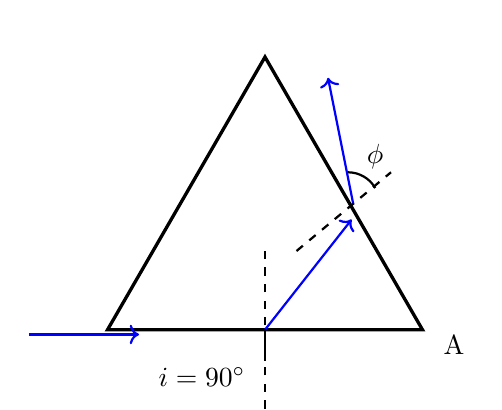
\begin{tikzpicture}[scale=2]
        % Draw prism
        \draw[very thick] (0,0) -- (2,0) -- (1,1.732) -- cycle;
        
        % Draw incident and refracted rays
        \draw[thick][blue][->] (-0.5,-0.03) -- (0.2,-0.03);
        \draw[thick][blue][->] (1.0,0) -- (1.55,0.7);
        \draw[thick][blue][->]  (1.56,0.8)  -- (1.4,1.6); 
        % Draw normal
        \draw[thick][dashed] (1,-0.5) -- (1,0.5);
        \draw[thick][dashed] (1.2,0.5) -- (1.8,1);
        % Draw angles
        \draw [thick](1.7,0.9) arc (30:90:0.2);
        \draw (1.7,1.1) node {$\phi$};
        \draw (0.8,0) -|  (1,-0.2) ;
        \draw (0.6,-0.3) node {$i=90^{\circ}$};
        % Add labels
        \draw (2.2,-0.1) node {A};
    \end{tikzpicture} 
    \caption{掠入射法原理图}
\end{figure}

根据实验数据，极限角$\phi$的测量结果和不确定度如下：\\
\begin{equation*}
    \begin{aligned}
        \overline{\phi} &= \frac{41^{\circ}24' + 41^{\circ}26' + 41^{\circ}25'}{3} = 41^{\circ}25' \\
        u_A(\phi) &= \sqrt{\frac{\sum_{i=1}^3(\phi_i-\overline{\phi})^2}{n(n-1)}} = \frac{1'}{\sqrt{3}} 
    \end{aligned}
\end{equation*}
\quad $\phi$总的不确定度:
\begin{equation*}
    u_\phi = \sqrt{u_A^2 + u_{B1}^2} = \sqrt{\frac{1'}{\sqrt{3}}^2 + \frac{1'}{\sqrt{3}}^2} \approx 49'' 
\end{equation*}
\quad 由此计算三棱镜的折射率:
\begin{equation*}
\begin{aligned}
 n&=\sqrt{1+(\frac{cos\, A+sin\, \phi}{sin\, A})^2}=1.6689 \\
 u_n&=\sqrt{(\frac{(sin\, \phi+cos\,A)(1+sin\,\phi\ cos\,A)}{sin^3 \,A\sqrt{1+(\frac{cos\, A+sin\, \phi}{sin\, A})^2}}u_A)^2+(\frac{cos\,\phi(cos\,A+sin\,\phi)}{sin^2\,A\sqrt{1+(\frac{cos\, A+sin\, \phi}{sin\, A})^2}}u_\phi)^2}\\
    &=0.0003
\end{aligned}
\end{equation*}
\quad 最终测量结果：
\begin{equation}
    n = 1.6689 \pm 0.0003
\end{equation}

\subsection{最小偏向角测量三棱镜折射率}
\vspace{0.2cm}
\quad 采用汞灯作为光源，测量三棱镜对汞灯绿谱线$\lambda=546.07\,nm$的折射率,实验测量数据如下：
\begin{table}[H]
    \centering
    \begin{tabular}{cccccc}
        序号 & $\theta_5'$     & $\theta_5''$     & $\theta_6'$      & $\theta_6''$     & $\delta_m $                  \\ \hline
        1  & $6^{\circ}44'$ & $186^{\circ}43'$ & $60^{\circ}49'$ & $240^{\circ}47'$ & $54^{\circ}4'30''$     \\
        2  & $344^{\circ}34'$($-360^{\circ}$) & $164^{\circ}34'$ & $38^{\circ}38'$ & $218^{\circ}37'$ & $54^{\circ}3'30''$     \\
        3  & $32^{\circ}8'$ & $22^{\circ}8'$ & $86^{\circ}12'$ & $276^{\circ}12'$ & $54^{\circ}4'$
        \end{tabular}
    \caption{最小偏向角$\delta_m$（汞绿光）测量数据}
\end{table}
\begin{figure}[H]
    \centering
    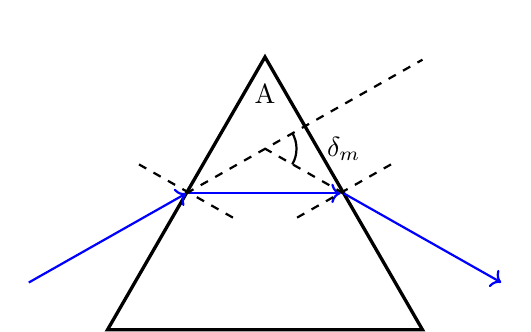
\begin{tikzpicture}[scale=2]
        % Draw prism
        \draw[very thick] (0,0) -- (2,0) -- (1,1.732) -- cycle;
        
        % Draw incident and refracted rays
        \draw[thick][blue][->] (-0.5,0.3) -- (0.5,0.866);
        \draw[thick][blue][->] (0.52,0.866) -- (1.48,0.866);
        \draw[thick][blue][->]  (1.5,0.866)  -- (2.5,0.3); 
        % Draw normal
        \draw[thick][dashed] (0.2,1.05) -- (0.8,0.71);
        \draw[thick][dashed] (1.8,1.05) -- (1.2,0.71);
        % Draw angles
        \draw [thick][dashed] (0.5,0.866)  -- (2,1.715);
        \draw [thick][dashed] (1.5,0.866)  -- (1,1.15);
        \draw (1.5,1.15) node {$\delta_m$};
        \draw [thick](1.1732,1.05) arc (-30:30:0.2);
        % Add labels
        \draw (1,1.5) node {A};
    \end{tikzpicture} 
    \caption{掠入射法原理图}
\end{figure}
根据实验数据，最小偏向角$\delta_m$的测量结果和不确定度如下：\\
\begin{equation*}
    \begin{aligned}
        \overline{\delta_m} &= \frac{54^{\circ}4'30'' + 54^{\circ}3'30'' + 54^{\circ}4'}{3} = 54^{\circ}4' \\
        u_A(\delta_m) &= \sqrt{\frac{\sum_{i=1}^3(\delta_{m_i}-\overline{\delta_m})^2}{n(n-1)}} = \frac{30''}{\sqrt{3}} 
    \end{aligned}
\end{equation*}
\quad  $\delta_m$总的不确定度:
\begin{equation*}
    u_{\delta_m} = \sqrt{u_A^2 + u_{B1}^2} = \sqrt{\frac{30''}{\sqrt{3}}^2 + \frac{1'}{\sqrt{3}}^2} \approx 39''
\end{equation*}
\quad 由此计算三棱镜的折射率:
\begin{equation*}
\begin{aligned}
 n&=\frac{sin\, \frac{A+\delta_m}{2}}{sin\, \frac{A}{2}}=1.6753 \\
\end{aligned}
%u=1.8816*10^-4
\end{equation*}
\quad 和对应的折射率不确定度:
\begin{equation*}
    \begin{aligned}
     u_n&=\sqrt{(\frac{sin\, \frac{\delta_m}{2}}{2\,sin^2\, \frac{A}{2}}u_A)^2+(\frac{cos\, \frac{A+\delta_m}{2}}{2\,sin\, \frac{A}{2}}u_{\delta_m})^2}\\
        &=0.0002
    \end{aligned}
    %u=1.8816*10^-4
    \end{equation*}
\quad 最终测量结果：
\begin{equation}
    n = 1.6753 \pm 0.0002
\end{equation}
\subsection{最小偏向角测量玻璃的色散曲线}
\vspace{0.2cm}
\quad 对于玻璃的色散曲线，我测量了汞灯可见谱线对应不同波长的最小偏向角并计算对应的折射率，实验数据如下：\\
\begin{table}[h]
    \centering
    \begin{tabular}{ccc}
    $\lambda/nm$ & $\delta_m$ & n \\ \hline
     404.66(暗紫)   &      $57^{\circ}36.5'$      &   1.7080\\
    435.84（蓝）         &    $56^{\circ}24'$        &  1.6970 \\
      546.07（绿）           &     $54^{\circ}4'$       &  1.6753\\
         576.96（黄）         &     $53^{\circ}39'$       &  1.6714 \\
            579.07（黄）          &    $53^{\circ}34'$        &   1.6705
    \end{tabular}
    \caption{最小偏向角测量数据}
\end{table}

\quad 根据实验数据，利用柯西公式拟合色散曲线$n=A+\frac{B}{\lambda^2}+\frac{C}{\lambda^4}$如下图:
\begin{figure}[h]
    \centering
    \includegraphics[width=0.8\textwidth]{dispersion.pdf}
    \caption{玻璃色散曲线}
\end{figure}

\quad 对应的拟合数据如下：
\begin{equation}
    \begin{aligned}
        A&=1.6457 \\
        B&=7.0505\times10^3\,nm^2 \\
        C&=5.1489\times10^8\,nm^4
    \end{aligned}
\end{equation}
\vspace{2cm}
\subsection{光栅常数的测定}
\vspace{0.2cm}
\quad 采用汞灯作为光源，测量光栅对汞绿光$\lambda=546.07\,nm$的$\pm2$级衍射角，实验数据如下：\\
\begin{table}[H]
    \centering
    \begin{tabular}{cccccc}
        序号 & $\theta_{+2}'$     & $\theta_{+2}''$     & $\theta_{-2}'$      & $\theta_{-2}''$     & $\phi_{\pm 2} $                  \\ \hline
        1  & $299^{\circ}30'$($-360^{\circ}$) & $119^{\circ}30'$ & $21^{\circ}21'$ & $201^{\circ}27'$ & $40^{\circ}57'$     \\
        2  & $22^{\circ}38'$ & $102^{\circ}44'$ & $104^{\circ}30'$ & $284^{\circ}38'$ & $40^{\circ}56'30''$     \\
        3  & $39^{\circ}18'$ & $219^{\circ}24'$ & $121^{\circ}12'$ & $301^{\circ}15'$ & $40^{\circ}56'15''$
        \end{tabular}
    \caption{光栅常数的测量数据}
\end{table}
根据以上数据，绿光的$\pm$2级衍射的测量结果和不确定度如下：\\
\begin{equation*}
    \begin{aligned}
        \overline{\phi_{\pm 2}} &= \frac{40^{\circ}57' + 40^{\circ}56'30'' + 40^{\circ}56'15''}{3} = 40^{\circ}56'35'' \\
        u_A(\phi_{\pm 2}) &= \sqrt{\frac{\sum_{i=1}^3(\phi_{\pm 2_i}-\overline{\phi_{\pm 2}})^2}{n(n-1)}} \approx 13'' 
    \end{aligned}
\end{equation*}
\quad $\phi_{\pm 2}$总的不确定度:
\begin{equation*}
    u_{\phi_{\pm 2}} = \sqrt{u_A^2 + u_{B1}^2} = \sqrt{13''^2 + \frac{1'}{\sqrt{3}}^2} \approx 37''
\end{equation*}
\quad 由此计算光栅常数:
\begin{equation*}
\begin{aligned}
 d&=\frac{2\, \lambda}{sin\,\phi_{\pm 2}}=1666.6\,mm \\  
\end{aligned}
\end{equation*}
\quad 和对应的光栅常数不确定度:
\begin{equation*}
    \begin{aligned}
     u_d&=\frac {2\, \lambda\, cos\,\phi_{\pm 2}}{sin^2\,\phi_{\pm 2}}u_{\phi_{\pm 2}}=0.4\,mm
    \end{aligned}
    %u=0.3446nm
    \end{equation*}
\quad 最终测量结果：
\begin{equation}
    d = 1666.6\,nm \pm 0.4\,nm
    %d = (1666.604041\pm 0.3446),nm
\end{equation}
\quad 对应的空间频率:
\begin{equation*}
\begin{aligned}
    f&=\frac{1}{d}=600.0\, mm^{-1}  \\
    u_f&=\frac{u_d}{d^2}=0.2\, mm^{-1}
\end{aligned}
\end{equation*}
\quad 最终测量结果：
\begin{equation}
    f = (600.0 \pm 0.2)\,mm^{-1}
\end{equation}
\vspace{1cm}
\subsection{测量汞灯双黄线波长和角色散率}
\vspace{0.2cm}
\quad 采用汞灯作为光源，测量汞灯双黄线（标准值：$\lambda_1=576.96\,nm$和$\lambda_2=579.07\,nm$）的$\pm1$级衍射角，实验数据如下：\\
\begin{table}[H]
    \centering
    \begin{tabular}{cccccc}
        序号 & $\theta_{+1}'$     & $\theta_{+1}''$     & $\theta_{-1}'$      & $\theta_{-1}''$     & $\phi_{\pm 1} $                  \\ \hline
        1  & $162^{\circ}21'$ & $342^{\circ}23'$($-360^{\circ}$) & $202^{\circ}52'$ & $22^{\circ}54'$ & $20^{\circ}15'30''$     \\
        2  & $194^{\circ}32'$ & $14^{\circ}34'$ & $235^{\circ}02'$ & $55^{\circ}04'$ & $20^{\circ}15'$     \\
        3  & $234^{\circ}47'$ & $54^{\circ}51'$ & $275^{\circ}17'$ & $95^{\circ}20'$ & $20^{\circ}14'45''$
        \end{tabular}
    \caption{汞灯黄谱线1的测量数据}
    \vspace{0.2cm}
    \begin{tabular}{cccccc}
        序号 & $\theta_{+1}'$     & $\theta_{+1}''$     & $\theta_{-1}'$      & $\theta_{-1}''$     & $\phi_{\pm 1} $                  \\ \hline
        1  & $200^{\circ}51'$ & $20^{\circ}53'$ & $241^{\circ}30'$ & $61^{\circ}30'$ & $20^{\circ}19'$     \\
        2  & $187^{\circ}39'$ & $7^{\circ}41'$ & $228^{\circ}20'$ & $48^{\circ}22'$ & $20^{\circ}20'30''$     \\
        3  & $227^{\circ}46'$ & $47^{\circ}48'$ & $268^{\circ}26'$ & $88^{\circ}28'$ & $20^{\circ}20'$
        \end{tabular}
    \caption{汞灯黄谱线2的测量数据}
\end{table}
根据以上数据，汞灯双黄线的$\pm$1级衍射的测量结果和不确定度如下：\\
\begin{equation*}
    \begin{aligned}
        \overline{\phi_{1}} &= \frac{20^{\circ}15'30‘’ + 20^{\circ}15 + 20^{\circ}14'45''}{3} = 20^{\circ}15'5'' \\
        \overline{\phi_{2}} &= \frac{20^{\circ}19' + 20^{\circ}20'30'' + 20^{\circ}20'}{3} = 20^{\circ}19'50'' \\
        u(\phi_{1}) &= \sqrt{\frac{\sum_{i=1}^3(\phi_{1_i}-\overline{\phi_{1}})^2}{n(n-1)}+(\frac{\Delta}{\sqrt{3}})^2} \approx 37'' \\
        u(\phi_{2}) &= \sqrt{\frac{\sum_{i=1}^3(\phi_{2_i}-\overline{\phi_{2}})^2}{n(n-1)}+(\frac{\Delta}{\sqrt{3}})^2} \approx 44''
    \end{aligned}
\end{equation*}
\quad 进一步计算汞灯双黄线的波长和角色散率:
\begin{equation*}
\begin{aligned}
 \lambda_1&=d\,sin\,\phi_1=576.88\,nm \\
 \lambda_2&=d\,sin\,\phi_2=579.04\,nm \\
\end{aligned}
\end{equation*}
\begin{equation*}
\begin{aligned}
 u_{\lambda_1}&=\sqrt{((d\,cos\,\phi_1\,u(\phi_1))^2+(sin\,\phi_1\,u_d)^2}=0.30\,nm \\
 u_{\lambda_2}&=\sqrt{((d\,cos\,\phi_2\,u(\phi_2))^2+(sin\,\phi_2\,u_d)^2}=0.35\,nm \\
\end{aligned}
\end{equation*}
\quad 最终测量结果：
\begin{equation}
    \begin{aligned}
        \lambda_1 &=\, (576.88\, \pm 0.30)&nm \\
        \lambda_2 &=\, (579.04\, \pm 0.35)&nm \\
        \Delta \lambda&=\,\quad \quad \;2.16&nm
    \end{aligned}
\end{equation}
\quad 计算光栅的角色散率:
\begin{equation}
\begin{aligned}
 D&=\quad \;\; \frac{\Delta \phi}{\Delta \lambda}&=6.397\times 10^{-4}\,rad/nm \\
 D&=\quad \frac{k}{d\,cos\,\phi}&=6.397\times 10^{-4}\,rad/nm 
\end{aligned}
\end{equation}
\quad 可以发现，实验数据的角色散率与理论值相吻合，一致性较好，也和波长的标准值较为接近.

\subsection{测量光栅的分辨本领}
\vspace{0.2cm}
\quad 采用钠双黄线进行测量，测量在1级谱线恰好不能分辨时狭缝的宽度，计算得到光栅的分辨本领，实验数据如下：\\
\begin{table}[h]
    \centering
    \begin{tabular}{cccc}
    序号    & 1      & 2      & 3      \\ \hline
    $x_L$ & 19.369 & 17.958 & 14.700 \\
    $x_R$ & 17.809 & 16.400 & 13.116 \\
    D     & 1.560  & 1.558  & 1.584 
    \end{tabular}
    \caption{极限宽度D的测量(单位:mm)}
\end{table}

根据以上数据，得到极限狭缝宽度和此时的有效光栅条数:
\begin{equation*}
\begin{aligned}
\overline{D}&=\frac{1.560+1.558+1.584}{3}=1.567\,mm \\
N&=\frac{\overline D}{d}=940.2
\end{aligned}
\end{equation*}
\quad 最终测量结果，光栅的分辨本领为:
\begin{equation}
    R=kN=940.2
\end{equation}

比对理论值$R=\frac{\lambda}{\Delta_{\lambda}}=982.2$，两者大致相同，可见测量结果是合理的.

\section{实验结论与反思}
\quad 本次实验学习了分光计的调节，用极限角法和掠入射法测量了三棱镜的折射率，并拟合了玻璃的色散曲线。拓展实验测量了光栅的常数和分辨本领，测量了汞灯双黄线的波长和角色散率，实验结果与理论值基本吻合，实验结果较为准确一致性较好，实验过程中也学习了很多实验技巧和数据处理方法，总结了以下经验教训：
\begin{itemize}
    \item 粗调和目视观察是非常高效的实验方式，例如在寻找极限角时，肉眼观察分界线位置后再用望远镜精确读数，可以大大缩短实验时间；
    \item 在实际测量开始前进行预读数，以保证实验数据的正确性；并且不要给自己添加不必要的麻烦，比如一开始放置三棱镜时候就应该提前想到游标盘的位置，如果被平行光管挡住了就会大大增加后续测量过程的困难；
    \item 实验所用的方法：掠入射法、极限角法、分辨本领测量等，都是非常实用且精确的测量方法，这也离不开分光计仪器的高精度，但是需要保证实验条件，例如共轴，垂直入射等等的满足，才能使得测量更加精确。对于最后测量光栅分辨本领的实验，也是一种很好的实验方法，通过测量极限宽度，可以得到光栅的分辨本领，虽然肉眼判断有一定的主观性，不如定量测量精确，但是也能得到较为准确的结果。
\end{itemize}
\end{document}

